\documentclass[runningheads]{llncs}
\usepackage{graphicx}
\usepackage{amssymb,amsmath}
\usepackage{latexsym}
\usepackage{isabelle,isabellesym}

\newcommand{\equidom}[3]{{#1}\stackrel{#2}{\sim}{#3}}
\makeatletter
\newcommand{\superimpose}[2]
	{{\ooalign{$#1\@firstoftwo#2$\cr\hfil$#1\@secondoftwo#2$\hfil\cr}}}
\makeatother
\newcommand{\interf}{\leadsto}
\newcommand{\ninterf}{\mathrel{\mathpalette\superimpose{{\slash}{\leadsto}}}}

\begin{document}

\title{Formal Verification for A Buddy Allocation Model Specification}

\author{Ke Jiang\inst{1} \and
		Yongwang Zhao\inst{2,3} \and
		David San\'{a}n\inst{1} \and
		Yang Liu\inst{1}}

\authorrunning{Ke Jiang et al.}

\institute{School of Computer Science and Engineering, Nanyang Technological University, Singapore
	\and School of Computer Science and Engineering, Beihang University, Beijing, China
	\and Beijing Advanced Innovation Center for Big Data and Brain Computing, \\
	Beihang University, Beijing, China}

\maketitle


\begin{abstract}
Buddy allocation algorithms are widely adopted by memory management systems to manage the address space accessed by applications. However, errors in any stage of the development process of the memory management component, from the specification to the implementation, may lead to critical issues in other components using it. Rigorous mathematical proofs provide strong assurance to the development process. We apply formal methods to ensure the correctness in the specification of a buddy allocation algorithm. In this paper, we use the interactive theorem prover Isabell/HOL to construct a specification for a buddy allocation algorithm consisting on operations to allocate and dispose memory areas. Thence we verify that the operations preserve key invariants over the memory to guarantee functional correctness of the algorithm. Finally, we verify that the operations also preserve integrity of the memory, therefore they do not affect other memory areas previously allocated.

\keywords{Memory Specification \and
		Formal Verification \and
		Functional Correctness \and
		Security.}
\end{abstract}


\section{Introduction}
The correctness of applications and libraries of a system using dynamic memory allocation relies on properties the memory has to preserve. Errors in any stage of the development process of the memory management components, may break those properties, leading to critical issues in the rest of the system. Along the last decades, formal methods have been successfully applied to the verification of critical systems. To improve confidence on the reliability of a memory management, verification of functional correctness and security properties is applied from the top specification layers down to the implementation and the machine code.

Formal verification has been applied to memory managers going from very abstract models to more concrete ones. For instance, the work in\cite{reg_higham} formalized an abstraction of the memory management by a sequence of write and read operations. They proved the sequential consistency over this abstraction. Also focusing on a high level of abstraction, the work in\cite{reg_blazy} provided a memory model for an imperative language, defining the necessary memory operations for the language at both specification and implementation levels. It defined an axiomatic reasoning framework, proving that the memory semantics satisfies such axiomatic rules. In a similar way,\cite{reg_mansky} also provided an axiomatic proof system for a sequential memory model, which brings together an unified representation of the memory rules. In this sense, the work in\cite{reg_mansky} proved that their memory rules also satisfy the ones in\cite{reg_blazy}.

For the implementation level, the work from\cite{reg_marti} specified a heap manager from the implementation level directly and verified its functional correctness. It developed a library for separation logic to handle the pointers in C source codes and to ensure the separation of memory blocks. Another work from\cite{reg_mangano} specified and verified a memory allocation module of Contiki, where blocks are preallocated. The work specified C source codes of memory layouts, allocation and deallocation operations by Frama-C. Its verification detected errors like out-of-bounds accesses and potentially harmful situations by automatic provers like Frama-C/Wp. Also, work from\cite{reg_sahebolamri} formally verified the correctness of a heap allocator at source code level. The C source codes were translated into semantics language in Isabelle/HOL using CParser and AutoCorres. A specification consisting of allocation and deallocation operations was built and formally proved. The equality between semantics language and specification was also proved automatically.

Although an extensive number of works have formally specified and verified the abstract models and implementations of dynamic memory allocation, to our knowledge, litter work has been done to specify and verify buddy memory allocation. Our work is then such a work that to specify and verify the buddy memory allocation in algorithms level. The buddy memory allocation system was originally described by\cite{reg_knowlton}. It is widely used in many operating systems, in particular most versions of UNIX. For example, BSD\cite{reg_mckusick} uses this memory system for blocks smaller than a page, i.e., 4 kilobytes. The classic description of the buddy memory allocation system is released by\cite{reg_knuth}.

In this paper, we develop a specification for a buddy memory allocation algorithm in the Isabelle/HOL proof assistant. The algorithm provides applications with two services which are the allocation and disposal of memory blocks. Our specification consists of algorithm details as specific as possible for the sake of capturing all features in the algorithm. Then we specify and prove properties including explicit behavior expectations and correct memory layouts for functional correctness of the algorithm. Finally, we show that the memory services preserve integrity of other memory blocks which are previously allocated.

The paper is organized as follows. The second section briefly introduces the backgrounds of buddy memory allocation algorithms and Isabelle/HOL verification environment. The next section is about how we specify a buddy memory allocation model. The proofs to properties for functional correctness and the verification of integrity for security are arranged in the following section. The last section is about the conclusions and future work.

\section{Background}
In this section, we give necessary backgrounds for the buddy memory allocation algorithms and the Isabelle/HOL theorem prover.

\subsection{Buddy Allocation Algorithms}\label{sec:buddy}
The buddy allocation algorithms aim to minimize external fragmentation by partitioning the memory into blocks fitting as best as possible memory requests from applications. Starting from an initial block with capacity equal to the maximum available memory $\Omega$, blocks are split into a power-of-two number of blocks $\Gamma$ to ease address computation. Each of the split blocks are buddies of each other and will be coalesced into a single block whenever it is possible when disposing an allocated block.

This mechanism logically organizes the memory into levels, where each level $l$ hosts $\Gamma^l$ blocks of equal size $\Omega/{\Gamma}^l$. Assuming the maximum memory $\Omega$ is a constant, it is easy to show that the level containing blocks with the necessary capacity to satisfy a memory request of size $s$ is $\Delta_s \equiv \lceil log_\Gamma (\Omega / s) \rceil$ where $\lceil n \rceil$ is the upper natural number of $n$.

For efficiency when accessing the free available blocks of a given allocation request, implementations use a multilevel linked-list to manage the free blocks on a given level. Under an allocation request of size $s$, if the linked list for the level $\Delta_s$ is not empty, a block is directly picked from the head of list. If it is empty the mechanism will try to find a higher level with free blocks and the splitting process starts to generate a perfect fit for the requested size. 

When a block is deallocated, the algorithms check whether the block can be merged with its buddy blocks. Together with the list of free nodes of a level, the implementations keep a bitmap with the allocation state of the nodes of a level for quickly coalescing of free buddy nodes. Otherwise the coalescing algorithm would need to traverse the free node list of the level the coalesce is happening at to check that all the buddies blocks are in the list. On levels with a large number of free nodes using a bitmap can significantly increase the performance of the algorithm.

In this work, we provide a specification for the buddy allocator implemented in Zephyr, which uses quad-trees so $\Gamma = 4$. Fig.~\ref{fig3} represents the memory system using the multilevel free linked-list and the multilevel free bitmap with $\Gamma = 2$ to ease the representation. It is composed of three memory blocks at level 0 numerated from 0 to 2. Only the block 0 has allocated memory requests, and hence the multilevel free linked-list on level 0 only contains blocks 1 and 2. Allocated nodes 3 and 4 at level 1, and node 7 at level 2 are logical nodes, that is they do not represent physical addresses. Leaves at nodes 5, 6, 8, 9, and 10 do represent physical nodes that have been, or can be, allocated.

\begin{figure*}[htbp]
	\centering
	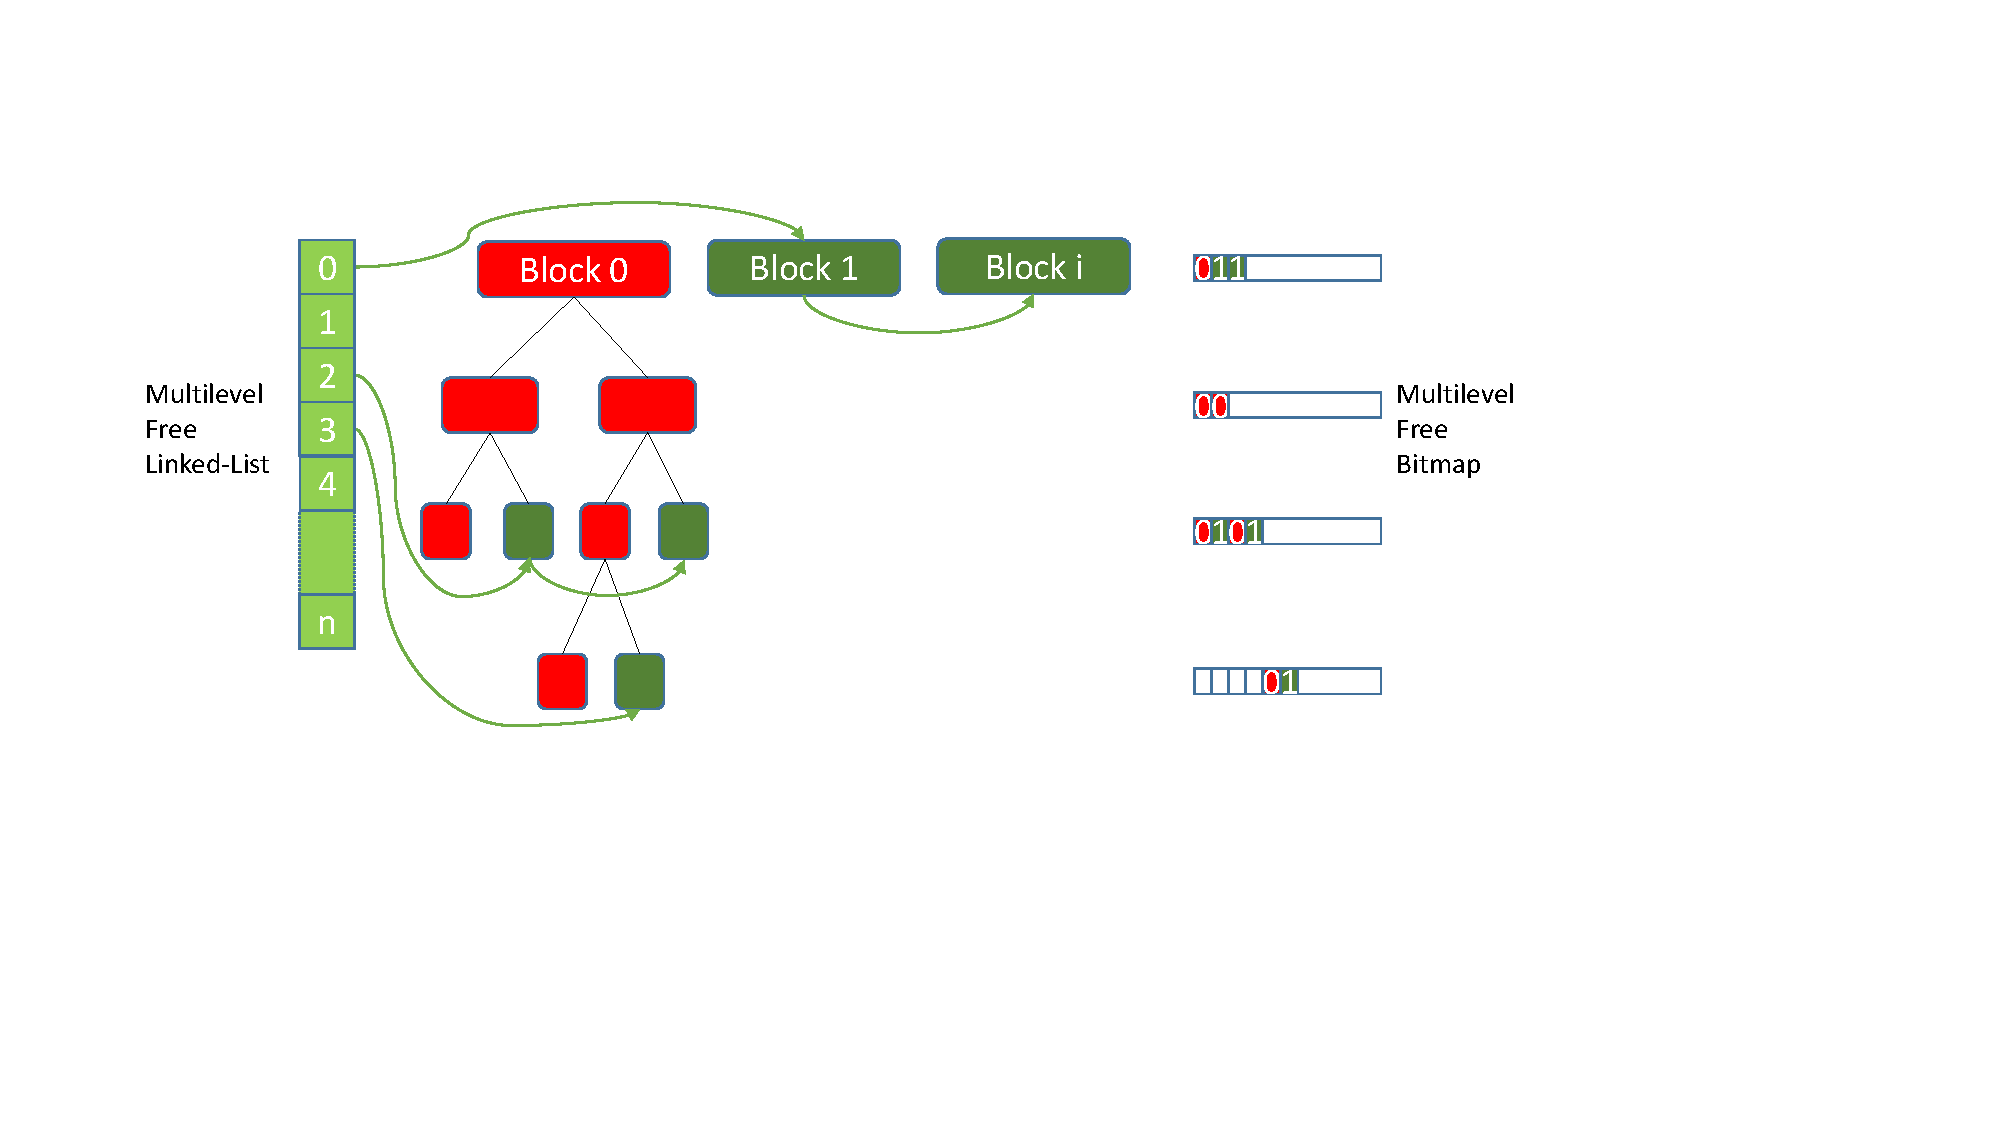
\includegraphics[width=0.8\textwidth]{fig3.pdf}
	\caption{Structures in Buddy Allocation Algorithms}
	\label{fig3}
\end{figure*}

\subsection{Isabelle/HOL}
We use the Isabelle/HOL interactive theorem prover~\cite{reg_Isabelle/HOL} to conduct the specification and verification of the memory management. Isabelle/HOL is a higher order logic theorem prover, using a typed lambda calculus-like functional language for specifications.

Isabelle/HOL includes a specification for simple common types such as naturals (\emph{nat}), integers (\emph{int}) and booleans (\emph{bool}). It also specifies some composed data types like tuples, records, lists and sets that are parametrized with other types. Isabelle provides the interface \emph{datatype} for the creation of user defined types based on type constructors.

Isabelle provides functions on predefined types to access their members or to provide additional operations over them. In the following we describe those functions and types that we use along this work. A tuple is denoted as (\emph{$t_1$} $\times$ \emph{$t_2$}), projection functions \emph{fst} and \emph{snd} respectively return elements $t_1$ and $t_2$. Lists are defined as a datatype with an empty construct denoted with \emph{NIL} or $[]$, and a concatenation construct denoted with $\#$, where $x\#xs$ adds $x$ to the front of $xs$. The $i$th component of a list $as$ is written as $as!i$. Isabelle/HOL provides functions for definite and indefinite descriptions. Definitive description is represented by $THE\ x.\ P\ x$ and returns the element uniquely described by the predicate $P$, else it returns and undefined value. Indefinite description is represented by $SOME\ x.\, P\ x$, selecting a random element from the predicate $P$ that must describe at least one element, else it returns an arbitrary value. The function $Card\ s$, denoted as $|s|$, returns the cardinality of the set $s$ when $s$ is finite, or $0$ when $s$ is infinite.

Isabelle/HOL allows users to create non-recursive specifications using the command \emph{definition}, and to create recursive specifications using commands \emph{primrec} and \emph{recursive}.

\begin{figure*}[htbp]
	\centering
	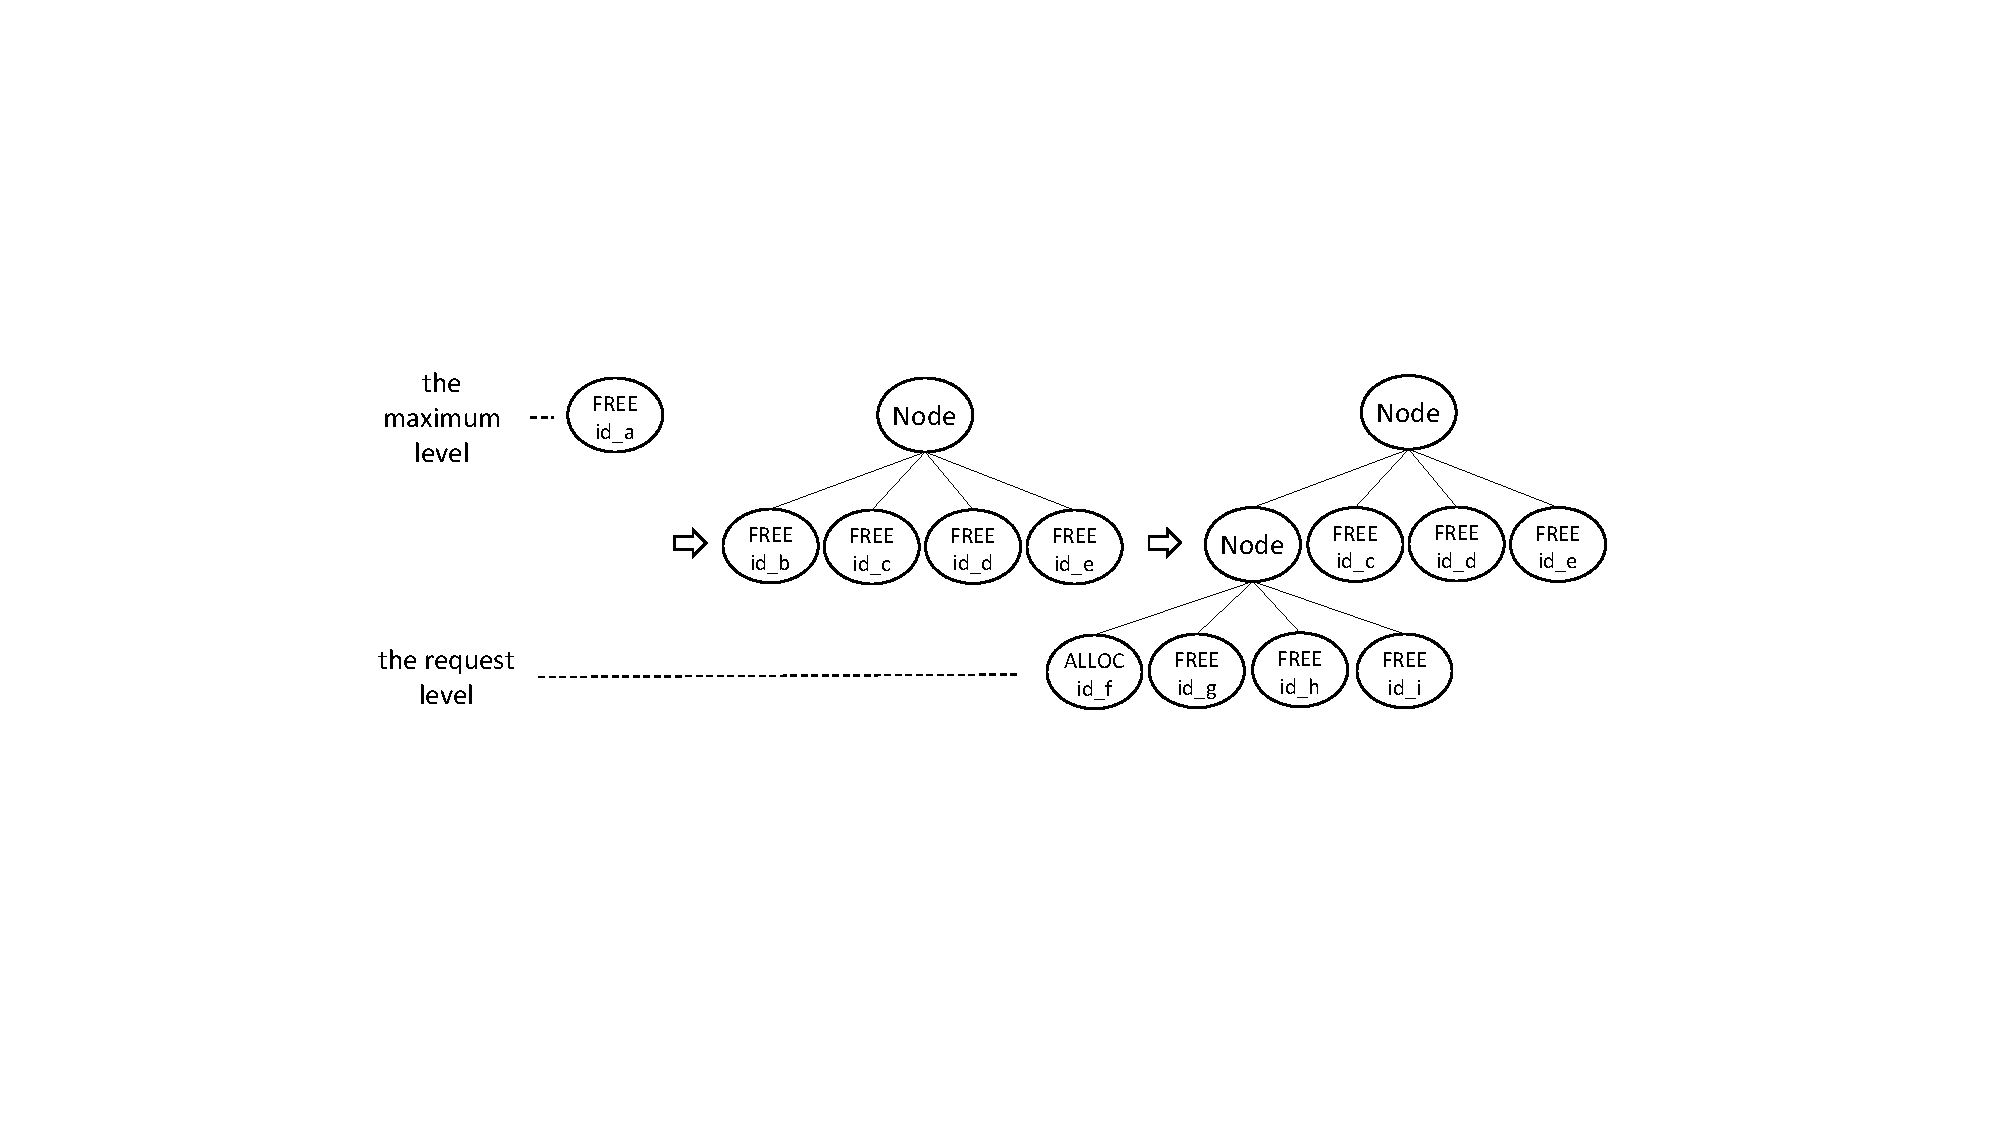
\includegraphics[width=0.7\textwidth]{fig1.pdf}
	\caption{The progress of dividing a free leaf}
	\label{fig:splitleaf}
\end{figure*}

\section{Specification of Buddy Allocation Model}\label{sec:spec}
The specification of the buddy memory allocation consists of a model for the necessary data structures to represent the memory layout, as well as a model for the allocation and disposal operations. This specification follows the algorithm for the buddy memory management in Zephyr OS, which applies a quartering split over blocks.

\subsection{State Representation}\label{statedes}
In the specification, the state models the memory as a set of quad-trees, each of them representing a memory pool. At this level of the specification, we assume that applications work with our block entity, so requesting a memory block returns the block itself, which will be used later during the deallocation.
\begin{align*}
(set:\ 'a)\ tree\ =\ &Leaf\ (L:\ 'a)\ | \\
&Node\ (LL:\ 'a\ tree)\ (LR:\ 'a\ tree)\\
&\ \ \ \ \ \ \ \ (RL:\ 'a\ tree)\ (RR:\ 'a\ tree)
\end{align*}

We define the structure of a quad-tree inductively. A quad-tree is parametrized by a variable type $'a$ and it has two constructors: \emph{Leaf} and \emph{Node}. A \emph{Leaf} is a terminal node storing values of the parametrized type $'a$, and a \emph{Node} has four (sub)trees that are built recursively. Notations \emph{LL}, \emph{LR}, \emph{RL} and \emph{RR} return the corresponding subtrees of the \emph{Node} tree. The notation \textbf{set} represents a function that gathers values of the parametrized type $'a$ from all \emph{Leaf} nodes.

In this specification, we use the tuple (\emph{block\_state\_type} $\times$ \emph{ID}) to instantiate the polymorphic type \emph{'a} in the quad-tree structure. Type \emph{block\_state\_type} indicates the usage state of a block and it is constructed using an Isabelle/HOL \emph{datatype}. It consists of two subtypes: \emph{ALLOC} and \emph{FREE}. The former is used to mark memory blocks that have been allocated to applications, whilst the latter is used to mark those unallocated blocks (hence they are free to be assigned to applications requesting memory). The type \emph{ID} is a natural number representing the address identifier of a memory block. Finally, the type \emph{BlockTree} represents an instantiated quad-tree in which terminal nodes represent allocated or free memory blocks identified by a natural number. We will indistinctively use the term of \emph{Leaf} as memory block along the document.
\begin{align*}
block\_state\_type\ &=\ FREE\ |\ ALLOC \\
ID\ &=\ nat \\
BlockTree\ &=\ (block\_state\_type\ \times\ ID)\ tree
\end{align*}

The allocation and free services are defined as a number of operations over the \emph{quad-tree} data structure representing the memory. These operations manipulate a \textsl{BlockTree}, accessing and modifying its structure and the data it stores. The function \textbf{level} takes two \emph{BlockTree}: \emph{btree} and \emph{b}, and it returns a natural number that represents the layer number where \emph{b} is located in \emph{btree} from the root node. The level of a node with regards to itself is $0$, and if $b$ does not belongs to $btree$, the function also returns $0$. We use the definitions \textbf{free\_lvl} and \textbf{alloc\_lvl}, which take a \emph{Blocktree} \emph{btree} and a natural number $l$, to respectively obtain the set with all the free and allocated \emph{Leaf} nodes located at level $l$ in \emph{btree}. We use the notation \emph{idset} to represent the collection of all used \emph{IDs}. To create a new Leaf node, we pick up as new \emph{ID} any natural number not belonging to \emph{idset}.

\subsection{Allocation Model}

\begin{definition} [Allocation Operation]
\begin{flalign*}
&alloc\ bset\ \Delta_s \triangleq \\
&if\ exists\_freelevel\ bset\ \Delta_s\ then \\
&\ \ \ \ lmax = freesets\_ml\ bset\ \Delta_s \\
&\ \ \ \ btree = SOME\ b.\ b \in bset \wedge free\_lvl\ b\ \Delta_s \ne \emptyset \\
&\ \ \ \ le = SOME\ l.\ l \in free\_lvl\ btree\ \Delta_s \\
&\ \ \ \ if\ lmax = \Delta_s\ then \\
&\ \ \ \ \ \ \ \ btree' = replace\ btree\ le\ (set\_type\ le\ ALLOC) \\
&\ \ \ \ \ \ \ \ return\ (bset - \lbrace btree \rbrace \cup \lbrace btree' \rbrace,\ True) \\
&\ \ \ \ else \\
&\ \ \ \ \ \ \ \ btree' = replace\ btree\ le\ (split\ le\ (\Delta_s - lmax)) \\
&\ \ \ \ \ \ \ \ return\ (bset - \lbrace btree \rbrace \cup \lbrace btree' \rbrace,\ True) \\
&else\ return\ (bset,\ False)
\end{flalign*}
\end{definition}

The allocation takes as input a set of quad-trees representing the available memory pools $bset$, and a natural number $s$ representing the requested size of the memory to allocate. If $s$ is bigger than the maximum size $\Omega$ for any memory pool, then the allocation fails and the state is not modified. If $s$ is smaller or equal than $\Omega$, then it calls function \textbf{alloc} over $bset$ and the level $\Delta_s$ containing blocks of size bigger or equal to $s$, as defined in Section~\ref{sec:buddy}. Function \textbf{alloc} carries out the necessary operations to find a block of size bigger or equal than $s$, and conducts the necessary modifications on $bset$ as we describe below.

\begin{figure*}[htbp]
\centering
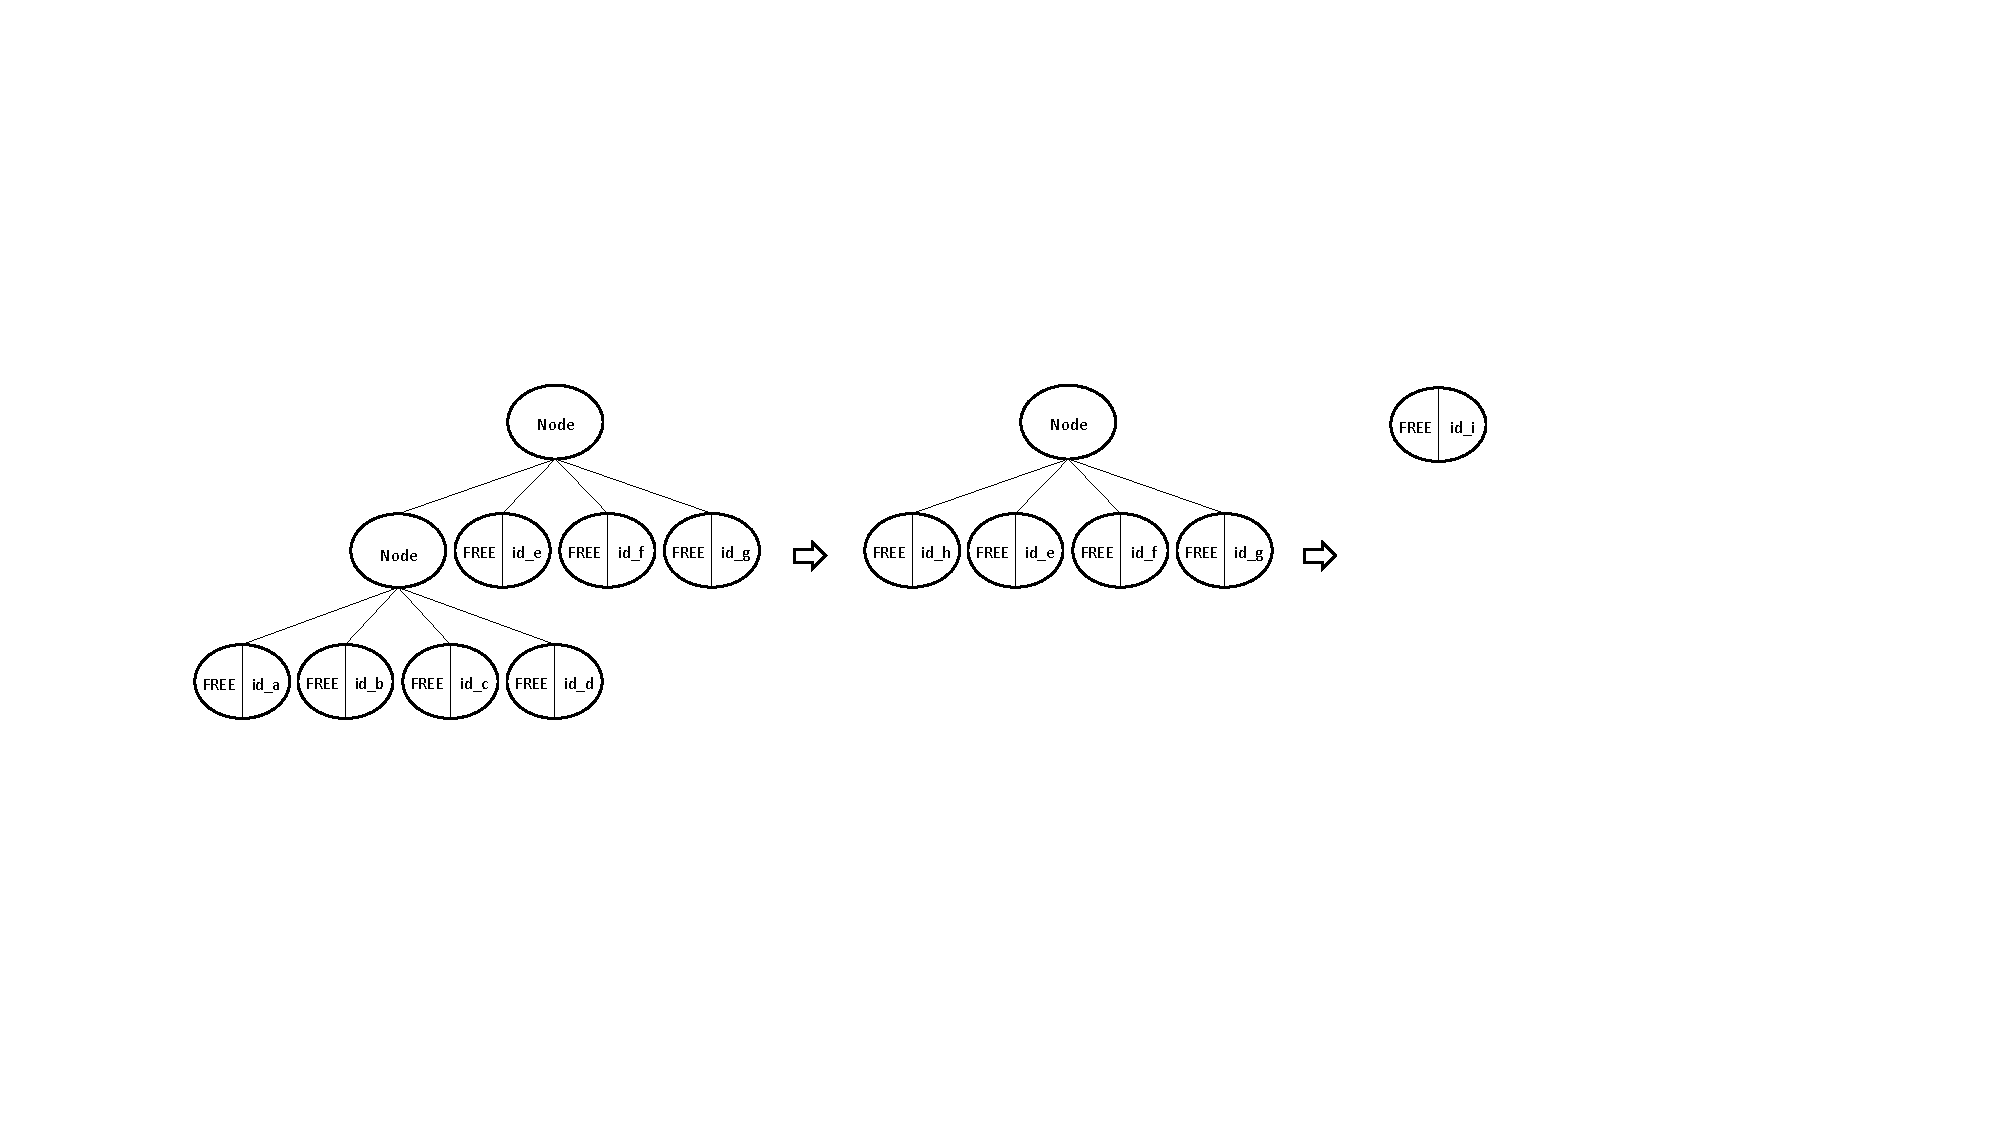
\includegraphics[width=0.7\textwidth]{fig2.pdf}
\caption{The progress of merging all free memory blocks}
\label{fig:merginfreeblocks}
\end{figure*}

%Alloc uses the predicate \textbf{exists\_freelevel}, with parameters $bset$ and $rlv$, to check if there exists a \emph{BlockTree} $b \in bsets$ and a level $l\leq rlv$ in $b$ such that $l$ has at least a free node.  and \textbf{freesets\_ml}. We first provide a description of these functions. Function \textbf{freesets\_ml} has the same inputs, and it returns the maximum level less or equal than $rlv$ for which it sets of free levels is not empty. Formally:
%
%\begin{definition} [Existence of Free Leaf Nodes]
%\begin{align*}
%exists&\_freelevel\ bset\ rlv \triangleq \\
%&\exists l\ b.\ l \leq rlv\ \wedge b \in bset \wedge free\_lvl\ b\ l \ne \emptyset
%\end{align*}
%\end{definition}
%
%\begin{definition} [Maximum Level of Free Leaf Nodes]
%\begin{align*}
%free&sets\_maxlevel\ bset\ rlv \triangleq THE\ lmax.\\
%&lmax \leq rlv\ \wedge \exists b \in bset.\ free\_lvl\ b\ lmax \neq \emptyset\ \wedge\\
%&(\forall l \leq rlv.\ \exists b \in bset.\ free\_lvl\ b\ l \ne \emptyset \longrightarrow \\
%&\ \ \ l \leq lmax)
%\end{align*}
%\end{definition}

%In addition, the allocation uses functions \textbf{set\_type}, \textbf{replace} and \textbf{replace\_leaf}. Function \emph{set\_type} takes a Leaf node \emph{b} and a target \emph{block\_state\_type} \emph{s} as inputs, and returns a leaf \emph{b'} resulting of changing the state of \emph{b} to \emph{s}. Function \emph{replace} takes a \emph{BlockTree} \emph{btree}, two Leaf nodes \emph{b} and \emph{b'} as inputs, and returns a tree replacing the Leaf node \emph{b} with \emph{b'} in \emph{btree}. Function \emph{replace\_leaf} takes a \emph{BlockTree} \emph{btree}, a Leaf node \emph{b} and a Node tree \emph{btr} as inputs, and returns the tree that replaces the Leaf node \emph{b} with \emph{btr} in \emph{btree}.

To allocate a block of size $s$ as described in Section~\ref{sec:buddy}, \textbf{alloc} firstly uses the predicate \textbf{exists\_freelevel}, which takes as input a set of \emph{BlockTree} $bset$ and the requested level $\Delta_s$ as parameters. \textbf{exists\_freelevel} checks whether there is a \emph{BlockTree} in \emph{bset} with free blocks at a level $l \leq \Delta_s$. If there is not, then the allocation process fails and returns the initial \emph{bset}. Otherwise, the function \textbf{freesets\_ml} takes $bset$ and $\Delta_s$ to return the maximum level $lmax \leq \Delta_s$ in $bset$ containing free blocks. The allocation procedure then gets a \emph{BlockTree} $btree$ from $bset$ such that there are free blocks at level $lmax$ and it randomly picks up a free \emph{Leaf} node $le$ from $btree$ at the level $lmax$. From here there are two options:

(1) There is a \emph{BlockTree} with free nodes at the requested level. Thence $lmax$ is equal to the requested level $\Delta_s$, and blocks at level $lmax$ have the minimum size to allocate the requested amount of memory. In this case the splitting process is not necessary and the procedure simply sets the type of $le$ as \emph{ALLOC} in $btree$, using the functions \textbf{set\_type} and \textbf{replace}, to obtain a new \emph{BlockTree} $btree'$. After that, the allocation returns an updated $bset$ by replacing the previous $btree$ with $btree'$. Note that this execution branch does not add any additional node into the tree structure, and only modifies the type of a terminal node at level $\Delta_s$.

(2) There is not a \emph{BlockTree} with free nodes at the requested level, and hence $lmax$ is smaller to the requested level $\Delta_s$. During the allocation process, if there is not any free \emph{Leaf} node available at the best fit level $\Delta_s$ for the requested size, but there exists a higher level $hl$ in the tree structure, hence $hl < \Delta_s$, with free blocks, it is necessary to start the splitting process from $hl$ down to $\Delta_s$. Fig.~\ref{fig:splitleaf} describes this process. The function \textbf{split} recursively divides a \emph{Leaf} node \emph{b} into a \emph{Node} tree \emph{btree} for $l - hl$ times. It uses the function \textbf{divide} that takes a Leaf node \emph{b} and returns a new non-terminal \emph{Node} tree \emph{n} with four terminal \emph{Leaf} nodes. The division operation is always conducted on the leftmost subtree of $n$ marking it as \emph{ALLOC}, while the rest are marked as \emph{FREE}. Therefore, the allocation replaces $le$ in $btree$ with the resulting node of splitting $le$ as described, following the rest of the procedure as in the first case. We define the \emph{split} operation as follows.

\begin{definition} [Split a Leaf Node]
\begin{align*}
split\ b\ lv &\triangleq\ if\ lv = 0\ then\ b\ else\\
Node\ &(split\ (LL\ divide\ b)\ (lv - 1))\ (LR\ divide\ b)\\ 
&(RL\ divide\ b)\ (RR\ divide\ b)
\end{align*}
\end{definition}

Note that \textbf{alloc} modifies a free block into an allocated one, so the number of leaves remain unmodified in the branch; or breaks a free block into a \emph{Node} tree to eventually create a number of free blocks and an allocated block as shown in Fig.~\ref{fig:splitleaf}. In both cases the rest of Leaves from the original set do not change and there is a new allocated block that was not contained in the set of allocated blocks of the initial tree. To obtain the block \textbf{alloc} allocates, it is only necessary to subtract the allocated nodes in the original set of free nodes from the allocated nodes in the resulting set.

\subsection{Deallocation Model}
The deallocation process takes a \emph{Leaf} node $b$ and a set of \emph{BlockTree} $bset$, and sets the state of $b$ to \emph{FREE}. During the deallocation process, if the state of all the buddies of $b$ is already $free$ and the level $l$ of $b$ is not the root node, the buddy nodes are merged to avoid fragmentation. The merging process is shown in Fig.~\ref{fig:merginfreeblocks}. During the merging process, $b$ and its buddies are removed, and the parent \emph{Node} of $b$ is transformed into a \emph{Leaf} node at level $l - 1$ that is set as free.

The function \textbf{free} firstly checks whether there is a $btree \in bset$ where $b$ belongs to and that its state is \emph{ALLOC}. If these conditions are not met, the procedure fails and returns the original \emph{bset}. If they are, the procedure picks up the tree \emph{btree} in \emph{bset} containing \emph{b}. Note that since leaves can only belong to one \emph{BlockTree}, $btree$ is unique. After this, \emph{btree} is modified into \emph{btree'} where the type of \emph{b} is set to \emph{FREE} using the functions \emph{set\_type} and \emph{replace}. After that, the new tree is coalesced using the function \textbf{merge}, and \emph{bset} is updated by replacing \emph{btree} with the new memory pool. The definition of deallocation operation is as follows.

\begin{definition} [Deallocation Operation]
	\begin{align*}
	&free\ bset\ b \triangleq \\
	&if\ \exists btree \in bset.\ b \in set\ btree\ then \\
	&\ \ \ \ if\ fst\ b = FREE\ then \\
	&\ \ \ \ \ \ \ \ return\ (bset,\ False) \\
	&\ \ \ \ else \\
	&\ \ \ \ \ \ \ \ btree = THE\ t.\ t \in bset \wedge b \in set\ t \\
	&\ \ \ \ \ \ \ \ btree' = replace\ btree\ b\ (set\_type\ b\ FREE) \\
	&\ \ \ \ \ \ \ \ btree'' = merge\ btree' \\
	&\ \ \ \ \ \ \ \ return\ (bset - \lbrace btree \rbrace \cup \lbrace btree'' \rbrace,\ True) \\
	&else\ return\ (bset,\ False)
	\end{align*}
\end{definition}

At this point, we have finished the specification of the allocation and disposal operations for a buddy memory allocator. 
\section{Verification}
In this section we will show that the formal specification introduced in the previous section preserves a set of properties guaranteeing its functional correctness in Section~\ref{sec:functional}. As a security property, we also prove that the specification preserves integrity of the memory structures in Section~\ref{sec:securitymodel} and Section~\ref{sec:securityproof}.
All the lemmas and theorems present in this section have been proven in the Isabelle/HOL theorem prover. We omit the proofs due to lack of space, but the interested reader can access the mechanize proofs in the project website~\footnote{www.ntu.securify.es/buddyallocator}

\subsection{Functional correctness}\label{sec:functional}
We first formulate and prove the desired properties for the allocation and deallocation services with regards to preservation of the memory layout. Note that models for \textbf{alloc} and \textbf{free} return a tuple $(BlockTree \times Bool)$, where the first element is the new memory layout, and the second one indicates the success or failure of the function. For simplicity on the presentation of the lemmas we consider that the models only return the new state of the memory layout.
\subsubsection{Allocation}\label{sec:functionalalloc}

We first show that the allocation service does not change the state when none of the memory pools in a set $b\_set$ have any free block big enough to allocate a request of size $rs$. 

\begin{lemma} [Allocation Failure]
\label{lemma:no_free_space}
\end{lemma}
\vspace{-7pt}
{\footnotesize
\begin{align*}
\neg exists\_freelevel\ b\_set\ \Delta_{rs} \longrightarrow (alloc\ b\_set\ \Delta_{rs}) = b\_set
\end{align*}
}
\vspace{-12pt}

As described in Section~\ref{sec:buddy} to allocate a memory block of size $rs$, there must be a free block on a level lower or equal than $\Delta_{rs}$. So under the assumption that there does not exist such a block, the allocation procedure leaves the state unchanged.

Then we show that if there is a memory pool with a block big enough to allocate the requested size $rs$, then \textbf{alloc} adds an allocated block at level $\Delta_{rs}$. We first split the lemma in two cases. The first case to the case in which level $\Delta_{rs}$ has free blocks, and hence the free block is not split but modified, it is shown in lemma~\ref{lemma:free_min2}. The second case is when $\Delta_{rs}$ does not have free blocks, and hence a free block in a level $l < \Delta_{rs}$ is split till reach level $\Delta_{rs}$ and it is shown in lemma lemma~\ref{lemma:free_nomin}.

%Then Lemma~\ref{pp2} and~\ref{pp3} respectively describe a transition during a direct allocation process. It says that the \emph{FREE} Leaf node which is to be allocated no longer belongs to free sets, and is a part of allocated sets. A direct allocation precess means that the existence of such a Block tree in \emph{b\_set}, the levels of whose \emph{FREE} leaf nodes are less than or equal to the value of \emph{rlv}. In particular, the maximum level among these \emph{FREE} leaf nodes is equal to the value of \emph{rlv}. Therefore, the function picks up a \emph{FREE} Leaf node in level \emph{rlv} to allocate.


\begin{lemma} [Allocsets for Direct Allocation]
\label{lemma:free_min2}
\end{lemma}
\vspace{-7pt}
{\footnotesize
\begin{align*}
&exists\_freelevel\ b\_set\ \Delta_{rs} \wedge freesets\_maxlevel\ b\_set\ \Delta_{rs} = \Delta_{rs}\longrightarrow\\ 
& \exists l.\ l \notin allocsets\ b\_set\ \wedge l \in allocsets\ (alloc\ b\_set\ \Delta_{rs}) \wedge  \\
&\ \ \ \ \ \ \ allocsets\ (alloc\ b\_set\ \Delta_{rs}) = allocsets\ b\_set \cup \lbrace l \rbrace) \wedge  \\
&\ \ \ \ \ \ \ level (alloc\ b\_set\ \Delta_{rs})\ l = \Delta_{rs}
\end{align*}
}
\vspace{-12pt}

%Lemma~\ref{pp4} introduces a transition during an indirect allocation process. The precondition preserves the existence of such a Block tree in \emph{b\_set}, that the levels of whose \emph{FREE} Leaf nodes are less than or equal to the value of \emph{rlv}. However, the maximum level among these \emph{FREE} Leaf nodes is less than the value of \emph{rlv}. With this precondition, function \emph{split} is invoked to divide a bigger Leaf node into small Leaf nodes until a Leaf node appears which satisfies the request. Then postcondition guarantees that a new Leaf node is added into the allocated set, while it dose not belong to this set previously.

\begin{lemma} [Allocsets for Indirect Allocation]
\label{lemma:free_nomin}
\end{lemma}
\vspace{-7pt}
{\footnotesize
\begin{align*}
&exists\_freelevel\ b\_set\  \Delta_{rs} \wedge freesets\_maxlevel\ b\_set\  \Delta_{rs} \neq  \Delta_{rs} \longrightarrow  \\
&\exists l.\ l \notin allocsets\ b\_set \wedge l \in allocsets\ (alloc\ b\_set\  \Delta_{rs}) \wedge \\
&allocsets\ (alloc\ b\_set\  \Delta_{rs}) = allocsets\ b\_set \cup \lbrace l \rbrace  \\
&\ \ \ \ \ \ \ \wedge level (alloc\ b\_set\ \Delta_{rs})\ l = \Delta_{rs} 
\end{align*}
}
\vspace{-12pt}

From lemmas~\ref{lemma:free_min2} and~\ref{lemma:free_nomin} we show the final lemma on the functional correctness of \textbf{alloc} with regards to allocated memory blocks. 

\begin{lemma} [Allocsets]
	\label{lemma:free}
\end{lemma}
\vspace{-7pt}
{\footnotesize
	\begin{align*}
	&exists\_freelevel\ b\_set\  \Delta_{rs} \longrightarrow  \\
	&\exists l.\ l \notin allocsets\ b\_set \wedge l \in allocsets\ (alloc\ b\_set\  \Delta_{rs}) \wedge \\
	&allocsets\ (alloc\ b\_set\  \Delta_{rs}) = allocsets\ b\_set \cup \lbrace l \rbrace  \\
	&\ \ \ \ \ \ \ \wedge level (alloc\ b\_set\ \Delta_{rs})\ l = \Delta_{rs} 
	\end{align*}
}
\vspace{-12pt}


For the allocation algorithm, we also show in lemma~\ref{lemma:free_alloc} that any free block in the initial set of memory pools $b\_set$, different than the block being allocated, remains free after allocation.

\begin{lemma} [Freeset for Allocation]
	\label{lemma:free_alloc}
\end{lemma}
\vspace{-7pt}
{\footnotesize
	\begin{align*}
	&exists\_freelevel\ b\_set\  \Delta_{rs} \wedge freesets\_maxlevel\ b\_set\  \Delta_{rs} \neq  \Delta_{rs} \longrightarrow  \\
	&\exists l.\ l \notin allocsets\ b\_set \wedge l \in allocsets\ (alloc\ b\_set\  \Delta_{rs}) \wedge \\
	& \forall l'. l'\neq l \wedge l' \in freesets\ b\_set \longrightarrow l' \in freesets (alloc\ b\_set\  \Delta_{rs}) 
	\end{align*}
}
\vspace{-12pt}


\subsubsection{Deallocation}\label{sec:functionalDealloc}
For deallocation, we first show in lemmas~\ref{lemma:deallocate_fail1} and~\ref{lemma:deallocate_fail2} that the deallocation service indeed does not change the memory layout when the block to deallocate does not belong to any memory pool in the memory layout, or when it exists but it has not been allocated. 


\begin{lemma} [Deallocation Failure 1]
\label{lemma:deallocate_fail1}
\end{lemma}
\vspace{-7pt}
{\footnotesize
\begin{align*}
\nexists btree \in b\_set.\ b \in set\ btree \longrightarrow (free\ b\_set\ b) = b\_set
\end{align*}
}
\vspace{-12pt}
	
\begin{lemma} [Deallocation Failure 2]
\label{lemma:deallocate_fail2}
\end{lemma}
\vspace{-7pt}
{\footnotesize
\begin{align*}
&\exists btree \in b\_set.\ b \in set\ btree \wedge fst\ b = FREE \\
&\longrightarrow (free\ b\_set\ b) = b\_set
\end{align*}
}
\vspace{-12pt}

Then we show in Lemma~\ref{lemma:deallocation} that the deallocation process carries out a correct transition during a deallocation success process. It describes that the Leaf node, which is to be released, dose not belong to allocated set any more.

\begin{lemma} [Allocsets for Deallocation]
\label{lemma:deallocation}
\end{lemma}
\vspace{-7pt}
{\footnotesize
\begin{align*}
&\exists btree \in b\_set.\ b \in set\ btree \wedge fst\ b \neq FREE \longrightarrow \\ 
& b\notin allocsets (free\ b\_set\ b) \wedge \\
& b\_set = allocsets\ (free\ b\_set\ b) \cup \lbrace b \rbrace
\end{align*}
}
\vspace{-12pt}

With regards to free blocks, the deallocation process may remove free memory blocks during the coercing procedure. However, we have to ensure that any free memory block after deallocating, different than the block resulting of the deallocation process, has to be also free in the initial set of free blocks $b\_set$. We show this in Lemma~\ref{lemma:freedealloc}.

\begin{lemma} [Freeset for Deallocation]
	\label{lemma:freedealloc}
\end{lemma}
\vspace{-7pt}
{\footnotesize
	\begin{align*}
	&\exists btree \in b\_set.\ b \in set\ btree \wedge fst\ b \neq FREE \longrightarrow \\ 
	&(1) \exists b'\ lvl.\ b' \in free\_lvl\ (free\ b\_set\ b)\ lvl \wedge b' \notin free_lvl (b\_set) lvl\ \wedge \\
	& (2) \forall b''. b''\neq b' \wedge b \in freesets (free\ b\_set\ b) \longrightarrow b'' \in b\_set
	\end{align*}
}
\vspace{-12pt}

This property first says that there is a free block $b'$ in the new set of memory pools that does not belong to the original set of memory pools (1). This is the free block resulting of deallocating the block. Then, we state that any other free block different than $b'$ belonging to the new set it also belongs to the original set (2).

%After giving these lemmas for preconditions and postconditions, we prove that our buddy allocation specification satisfies these behavior expectations. The first theorem we prove is as follows.
%
%\begin{theorem}
%The buddy allocation specification meets all behavior expectations described by preconditions and postconditions above.
%\end{theorem}

%Next, we introduce invariants to guarantee functional correctness of the specification from the memory layout perspective. Firstly, we ensure that the allocation operation picks out a correct and suitable Leaf node. Two properties are proved: the correctness of the function \emph{output\_level}, mapping the size of requested memory block to the level of the quad-tree in Definition~\ref{mostsuitable}; the correctness of the hierarchical structure in a quad-tree. Here are two lemmas that ensure the correctness of Definition~\ref{mostsuitable}.
%
%\begin{lemma} [Correctness of Function output\_level 1]
%\end{lemma}
%\vspace{-7pt}
%{\footnotesize
%\begin{align*}
%&\vert blo\_list \vert > 0 \wedge rsize \leq blo\_list\ !\ (\vert blo\_list \vert - 1) \\
%&\longrightarrow output\_level\ blo\_list\ rsize = \vert blo\_list \vert - 1
%\end{align*}
%}
%\vspace{-12pt}	
%
%\begin{lemma} [Correctness of Function output\_level 2]
%\end{lemma}
%\vspace{-7pt}
%{\footnotesize
%\begin{align*}
%&\vert blo\_list \vert > 1 \wedge l < \vert blo\_list \vert - 1 \\
%&\wedge rsize \leq blo\_list\ !\ l \wedge rsize > blo\_list\ !\ (l + 1) \\
%&\longrightarrow output\_level\ blo\_list\ rsize = l
%\end{align*}
%}
%\vspace{-12pt}
%
%With these two lemmas, we make sure the correctness of the mapping function \emph{output\_level}. 
\subsubsection{Correct Merging}
%We introduce a lemma to prove the correctness of the hierarchical structure of a quad-tree. It says that the level of root tree is zero, and the level of any child node is one more than its immediate father node. Function \textbf{root} checks whether the tree is a root tree, and function \textbf{child} gives us a set of all immediate child nodes of a Node tree.
%
%\begin{lemma} [Hierarchical Structure of a Quad-tree]
%\end{lemma}
%\vspace{-7pt}
%{\footnotesize
%\begin{align*}
%&(root\ btree \longrightarrow get\_level\ btree = 0) \\
%&\wedge (get\_level\ btree = l \wedge l \geq 0 \wedge chtree \in child\ btree \\
%&\ \ \ \longrightarrow get\_level\ chtree = l + 1)
%\end{align*}
%}	
%\vspace{-12pt}
%
%Until now, we have already proved the correctness of the mapping function \emph{output\_level} and the hierarchical structure of a quad-tree. Then we can deduce the following theorem to guarantee the property of picking out a correct and suitable Leaf node.
%
%\begin{theorem}
%The buddy allocation specification picks out a correct Leaf node and allocate it on the right level in the quad-tree.
%\end{theorem}

The buddy memory allocation algorithm may reduce the fragmentation by invoking merge function during the process of deallocation to merge buddy blocks that are free, as shown in Fig.~\ref{fig:merginfreeblocks}. Previous lemmas do not show that the merging procedure is correct, so we show here that the merging process is correctly carried out. This can be reduced to show that the memory layout preserves an invariant saying that buddy memory blocks are not all of them free. To achieve this, we first define the notion of all free buddy memory block using the definition below, where
function \textbf{child} gives us a set of all immediate child nodes of a \emph{Tree} and \textbf{leaf} is a predicate checking whether a node is terminal or not:
% In order to solve this, we still consider the correctness of the structure in a quad-tree during allocation and deallocation processes. We consider a fact that there is not such a Node tree, whose four immediate child nodes are all Leaf nodes and their types are \emph{FREE}. A definition is constructed as follows to check whether a quad-tree is such a Node tree. Function \textbf{leaf} is to check whether the tree is a Leaf node.

\begin{definition} [Four Free Leaves Belong to the Same Node] \label{def:FF4}
	\vspace{-7pt}
	{\footnotesize
		\begin{align*}
		is\_FFL\ btree \triangleq\ &\forall chtree \in child\ btree.\ leaf\ chtree \\
		&\wedge fst\ chtree = FREE
		\end{align*}
	}
\end{definition}

Operating system initialize the whole memory into a series of free blocks in different sizes, and these memory blocks are in the form of root nodes which are not split at the very beginning. This initialization state satisfies not-existence of \emph{FFL} trees. Then according to Lemma~\ref{lemma:allocffl} and~\ref{lemma:deallocffl}, any state after initialization satisfies non-existence of \emph{FFL} trees no matter operating system performs allocation or deallocation operations. Therefore, we can make sure the whole memory system preserves this property. We have this theorem as follows. Furthermore, it proves that the buddy allocation specification reduces the fragmentation by merge operation.
We then show in Lemmas~\ref{lemma:allocffl} and~\ref{lemma:deallocffl} that after the allocation and deallocation procedures there are no buddy groups where all the members are free. 

\begin{lemma} [Non-existence of FFL during Allocation]
\label{lemma:allocffl}
\end{lemma}
\vspace{-7pt}
{\footnotesize
\begin{align*}
\forall b \in b\_set.\ &\neg\ is\_FFL\ b \\
&\longrightarrow \forall b \in fst\ (alloc\ b\_set\ rlv).\ \neg\ is\_FFL\ b
\end{align*}
}
\vspace{-12pt}

\begin{lemma} [Non-existence of FFL during Deallocation]
\label{lemma:deallocffl}
\end{lemma}
\vspace{-7pt}
{\footnotesize
\begin{align*}
\forall b \in b\_set.\ &\neg\ is\_FFL\ b \\
&\longrightarrow \forall b \in fst\ (free\ b\_set\ b).\ \neg\ is\_FFL\ b
\end{align*}
}
\vspace{-12pt}

%We consider such a situation: operating system initialize the whole memory into a series of free blocks in different sizes, and these memory blocks are in the form of root nodes which are not split at the very beginning. This initialization state satisfies not-existence of \emph{FFL} trees. Then according to Lemma~\ref{allocffl} and~\ref{deallocffl}, any state after initialization satisfies non-existence of \emph{FFL} trees no matter operating system performs allocation or deallocation operations. Therefore, we can make sure the whole memory system preserves this property. We have this theorem as follows. Furthermore, it proves that the buddy allocation specification reduces the fragmentation by merge operation.
%
%\begin{theorem}
%The buddy allocation specification guarantees non-existence of FFL trees among all memory blocks.
%\end{theorem}

%\subsection{Security Properties}
%Regarding to security, we prove two important properties: memory isolation and non-leakage. The first one ensures non-overlapping of the address space allocated. The second one protect the integrity of the address space, ensuring that the memory domain is constant, i.e., the union of the sets of allocated memory blocks and free memory blocks is always the same.
%Another property non-leakage guarantees that available memory blocks (including occupied and free ones) are not getting less and less. In other words, it protects the integrity of address spaces.

\subsubsection{Memory Isolation}
Memory isolation ensures non-overlapping of the allocated address space. In Section~\ref{statedes} we show that the memory model uses a natural number as a block identifier \emph{ID}. The \emph{ID} helps us to uniquely identify each physical memory block in a memory pool. 

%We use that  \emph{ID} to represent the contiguous address occupied by a memory block. To link \emph{ID} to a real address, two things have to be introduced and proved: 1. a mapping function between a \emph{ID} and a real address as well as its correctness; 2. the one-to-one uniqueness between a \emph{ID} and a real address. We leave this part to the further work for a more detailed specification proof, in other words the design level of the buddy allocation. In this paper, we are not going to introduce real addresses into this specification, and we consider the correctness of the mapping function and promise its the uniqueness. Therefore, with these assumptions, isolation of address spaces means that all \emph{IDs} which Leaf nodes brings with are unique.

Definition~\ref{def:dif} introduces a judgment stating whether two Leaf nodes have the same \emph{ID}. This definition checks that for any memory pool $b$ in a memory layout $b\_set$, and any memory block $l$ in $b$, i.e. a terminal node of $b$, then there is not any other $l'$, different than $l$, and other memory pool $b'$ in $b\_set$ where the \emph{ID} of $l$ is equal the \emph{ID} of $l'$.

\begin{definition} [Different IDs]\label{def:dif}
{\footnotesize
	\begin{align*}
	&is\_different\ b\_set \triangleq \\
	&\forall b \in b\_set.\ \forall l \in set\ b.\ \nexists l'\ b'.\ l' \in set\ b' \wedge b' \in b\_set\ \wedge l' \ne l \wedge  \\
	&\ \ \ \ \ get\_id\ l' = get\_id\ l
	\end{align*}
}
\end{definition}

Lemmas~\ref{lemma:id_alloc} and~\ref{lemma:id_dealloc} shows that uniqueness of IDs is an invariant to the allocation and deallocation procedures.
%
%Lemmas~\ref{} that ensure this property holds during the procedures of allocation and deallocation if it holds in the assuming of implication expressions.

\begin{lemma} [Different IDs during Allocation] \label{lemma:id_alloc}
{\footnotesize
	\begin{align*}
	is\_different\ b\_set \longrightarrow is\_different\ fst\ (alloc\ b\_set\ rlv)
	\end{align*}
}
\end{lemma}


\begin{lemma} [Different IDs during Deallocation] \label{lemma:id_dealloc}
{\footnotesize
	\begin{align*}
	is\_different\ b\_set \longrightarrow is\_different\ fst\ (free\ b\_set\ b)
	\end{align*}
}
\end{lemma}


%Let us go back to the initialization state. The whole memory is divided into a finite number of free root nodes. We can easily guarantee that all \emph{IDs} these root nodes bring with are unique, and we initialize the collection \emph{idset} with these used \emph{IDs}. Then according to the lemmas above, any state after initialization satisfies \emph{Different IDs} no matter operation system performs allocation or deallocation operations. As a result, we can guarantee the whole memory system preserve \emph{Different IDs}. We have this theorem as follows.
%
%\begin{theorem}
%The buddy allocation specification ensures all IDs of Leaf nodes are unique.
%\end{theorem}

%Finally, with the assumptions that the correctness of the mapping function between a \emph{ID} and a real address, and promising its uniqueness, we prove the specification preserves the isolation of memory address spaces.

Considering that a block ID allows us to uniquely identify a memory block, the lemma on uniqueness of blocks and Lemma~\ref{lemma:free} allows to infer non-overlapping of allocation of memory blocks. That is, that two different allocations do not assign the same memory block.

Note that although our level of abstraction does not consider memory addresses, it would be easy to refine this model to include memory addresses and identify the domain of addresses of a memory block as a function in terms of the location of the memory block in the tree. 

%\subsubsection{Non-leakage of Memory Blocks}
%We use a quad-tree structure and map all the blocks into the Leaf nodes of these trees, thence the non-leakage means that all the Leaf nodes (including occupied and free ones) are recorded in use. If we can infer a correct and certain relation between the number of Leaf nodes and Non-leaf nodes of a quad-tree, we can prove that all the Leaf nodes are in use and none of them is forgotten. To achieve this, the first step is to search and prove a certain relation between the numbers of Leaf nodes and Non-leaf nodes in a quad-tree. Through exploration, we have found and proved such a relation as follows. Functions \textbf{get\_leaf} and \textbf{get\_node} take a Block and return Leaf nodes set and Non-leaf nodes set respectively.
%
%\begin{lemma} [Relation of a Quad-tree Nodes]
%\vspace{-7pt}
%\end{lemma}
%{\footnotesize
%\begin{align*}
%Qtree\ b:\ size\ (get\_leaf\ b) = size\ (get\_node\ b) \times 3 + 1
%\end{align*}
%}
%\vspace{-12pt}
%
%After establishing this relation, we use the following two lemmas to guarantee all the quad-trees during execution procedures maintain this relation.
%
%\begin{lemma} [Qtree during Allocation]
%\vspace{-7pt}
%\end{lemma}
%{\footnotesize
%\begin{align*}
%\forall b \in b\_set.\ Qtree\ b \longrightarrow \forall b \in fst\ (alloc\ b\_set\ rlv).\ Qtree\ b
%\end{align*}
%}
%\vspace{-12pt}
%
%\begin{lemma} [Qtree during Deallocation]
%\vspace{-7pt}
%\end{lemma}
%{\footnotesize
%\begin{align*}
%\forall b \in b\_set.\ Qtree\ b \longrightarrow \forall b \in fst\ (free\ b\_set\ b).\ Qtree\ b
%\end{align*}
%}
%\vspace{-12pt}
%
%In the end, we can prove that all quad-trees hold this relation between the number of Leaf nodes and Non-leaf nodes. The correct structure of a quad-tree means that all Leaf nodes (including occupied and free ones) are in use. We have this theorem as follows. Then considering the fact that all blocks are mapped into the Leaf nodes of these trees, we can ensure that the specification preserves memory non-leakage.
%
%\begin{theorem}
%The buddy allocation specification guarantees any Block is a Qtree.
%\end{theorem}
%
%To sum up, in this subsection we introduce preconditions and postconditions as well as significant invariants to ensure the formal buddy allocation specification preserves a set of properties which guarantee its functional correctness. In next two subsections, we build a security model and prove the specification preserves integrity of the memory structures.

\subsection{A Security Model}\label{sec:securitymodel}
Integrity is the assurance that information is trustworthy and accurate. To achieve this, data must not be changed in transit. In this subsection, we prove integrity of  the data allocated by a buddy allocation specification. For this purpose, we follow the work from~\cite{reg_securitymodel} to firstly design a security model, which consists of a nondeterministic state machine, and then to specify the integrity property and prove that it is an invariant on the memory allocator.

\subsubsection{Memory State Machine} 
We define a memory state machine as tuple $\mathcal{M} = \langle \mathcal{S}, \mathcal{E}, \varphi, s_0 \rangle$. $\mathcal{S}$ represents the state space,  $s_0 \in \mathcal{S}$ is the initial machine state, and $\mathcal{E}$ is the set of event labels. The state-transition function is characterized by $\varphi$, of type $\varphi: \mathcal{E} \rightarrow \mathbb{P}(\mathcal{S} \times \mathcal{S})$, where $\mathbb{P}(n)$ is the powerset of the set $n$.

Based on the state machine above, we introduce some auxiliary functions: function \textbf{execution(s, es)} takes a state \emph{s} and a sequence of events \emph{es}, then returns the set of final states; function \textbf{reachable(s)} (denoted as $\mathcal{R}(s)$) checks the reachability of a state \emph{s} from the initialized state $s_0$ by the \emph{execution} function: \emph{$\exists$es.\ s $\in$ execution($s_0$, es)}.

Next, we add the concept of domains, also referred as partitions, to represent the entities that execute the state-transition function. In addition, we introduce partition scheduling as a domain \textbf{scheduler}. Therefore, the domains ($\mathcal{D}$) in $\mathcal{M}$ are the configured partitions ($\mathcal{P}$) and the scheduler ($\mathbb{S}$), $\mathcal{D}$ = $\mathcal{P}$ $\cup$ $\lbrace$$\mathbb{S}$$\rbrace$.

\subsubsection{Integrity Definition} We use the notion of integrity from~\cite{reg_noninterference}, which provides a formalism for the specification of security policies. A domain \emph{u} is non-interfering with domain \emph{v} if no action performed by \emph{u} can influence the subsequence outputs seen by \emph{v}. We define the notion of integrity in our security model using the concepts of state equivalence and interfering.

Firstly, state equivalence is denoted as $\sigma_1 \sim \sigma_2$ is a relation in $(\mathbb{S}\times\mathbb{S})$. State equivalence of $\sigma_1$ and $\sigma_2$ on a domain $d$ is denoted as $\equidom{s}{d}{t}$.

Interference is a relation in $(\mathcal{D}\times\mathcal{D})$ and is denoted as $a \interf b$, representing that domain $a$ interfere with domain $b$. We use $a \ninterf b$ to express that a domain $a$ does not interfere domain $b$.



% In our security model, we forbid partitions to interfere with the \emph{scheduler}. Its aim is to ensure that \emph{scheduler} does not leak information by its scheduling decisions. Since the \emph{scheduler} can schedule other domains, it can interfere with them. However, the \emph{scheduler} cannot be interfered by any other domains to ensure that the \emph{scheduler} does not leak information by its scheduling decisions.

%With these two concepts, we can easily define the integrity property conditions as follows.
Integrity of an event $e$ is defined as:
\begin{definition} [Integrity] \label{def:integrity}
\vspace{-7pt}
\end{definition}	
{\footnotesize
\begin{align*}
integrity(e) \triangleq\ &\forall d\ s\ s'.\ \mathcal{R}(s) \wedge dom(s, e) \ninterf d \wedge (s, s') \in \varphi(e)\\
&\longrightarrow (\equidom{s}{d}{s'})
\end{align*}
}
\vspace{-12pt}

$dom(\sigma, e)$ is a function from pairs $(\mathcal{S}\times \mathcal{E})$ to $\mathcal{D}$, specifying the domain executing an event $e$ on a state $\sigma$. The notion of integrity states that for any domain $d$, and a reachable state $s$ from the initial state $s0$, if the domain executing the event $e$ in $s$ does not interfere with $d$, then for any state $s'$ that $e$ can transit to from $s$, $s$ is equivalent to $s'$ for the domain $d$. That is, if the domain executing $e$ is not able to interfere with $d$, then the execution of $e$ does not modify the information that domain $d$ observes.

\subsubsection{Security Model} We define the security model as:

\begin{definition} [Security Model] \\
{
The security model is a tuple \[\mathcal{S\_M} = \langle \mathcal{M}, \mathcal{D}, dom, \interf, \sim \rangle\] assuming the following assumptions.
\begin{enumerate}
\item $\forall$d $\in$ $\mathcal{D}$. $\mathbb{S}$ $\interf$ d
\item $\forall$d $\in$ $\mathcal{D}$. d $\interf$ $\mathbb{S}$ $\longrightarrow$ d = $\mathbb{S}$
\item $\forall$s t e. $\equidom{s}{\mathbb{S}}{t}$ $\longrightarrow$ dom(s, e) = dom(t, e)
\item $\forall$s e. $\mathcal{R}(s)$ $\longrightarrow$ $\exists$s'. (s, s') $\in$ $\varphi(e)$
\item $\forall$e. integrity(e)
\end{enumerate}
}
\end{definition}


The security model is tuple composed of a state machine $\mathcal{M}$, a set of execution domains $\mathcal{D}$, a function $dom$, and the relations for interference between domains and equivalence between states. The assumptions of the model represent that: the scheduler interfere with any execution domain (1); an execution domain $d$ cannot interfere with the scheduler, unless $d$ is the scheduler itself (2); two states $s$ and $t$ are equivalent on the scheduler only if the execution domain of $s$ and $t$ is the same on the execution of any event $e$ (3); any event $e$ be defined on any reachable state (4); all the events must preserve the integrity relation (5).

This security model constructs a sequential model for event-based specifications which ensures the preservation of the integrity  property for any possible execution trace on $\mathcal{M}$. In the next section, we instantiate the security model with our buddy allocation specification.

\subsection{Instantiation and Security Proofs}\label{sec:securityproof}
In this part, we construct an event specification by adding interfaces to the buddy allocation specification introduced in Section~\ref{sec:spec}. We instantiate the security model specifying the function for execution domains, and the relations of domain interference and state equivalence. We also prove that the wrapped buddy allocation events satisfy the integrity property.

\subsubsection{Instantiation}

We first define the notion of state used in the memory state machine $\mathcal{M}$ as $\Sigma = \langle \mathcal{MP}, \xi, \mathcal{A} \rangle$, where $\mathcal{MP}$ is a set of memory pools, i.e., the memory state; $\xi$ is the scheduled domain used to instantiate the function $dom$ in the security model; and $\mathcal{A}$ is a function from execution domains to memory blocks identifiers, which holds the memory blocks that have been allocated to each execution domain. We use  $\mathcal{A}$  to instantiate the equivalence function among domains.


The events $\mathcal{E}$ in the security model is a set composed of an allocation, deallocation, and scheduler event. The interfaces for the allocation and deallocation use the \emph{alloc} and \emph{free} functions defined in Section~\ref{sec:spec} to update the internal information of the memory and the blocks identifier used by the domain executing the event. The Scheduler is an event function that sets $\xi$ non-deterministically with any execution domain. Note that we constrain the execution of allocation and free functions to be carried out by an execution domain that is not the scheduler, and the execution of the scheduler by the scheduler domain. The transition relation is defined as:

\begin{definition} [Allocate Memory Interface]
{
\begin{align*}
\forall rlv&. \varphi\ allocate\_memory\ \Sigma \triangleq \\ 
&if\ snd\ (alloc\ (\mathcal{MS}\ \Sigma)\ rlv) = True\ \wedge \xi\ \Sigma \neq \mathbb{S}\ then \\
&\ \ \ \  \langle (alloc\ (\mathcal{MS}\ \Sigma)\ rlv), \xi, \mathcal{A}[\xi := \mathcal{A}\ \xi \\
&\ \ \ \ \ \ \ \cup \lbrace allocid\ (alloc\ (\mathcal{MS}\ \Sigma)\ rlv) \rbrace] \rangle \\
&else\ \Sigma
\end{align*}
}
\end{definition}

\begin{definition} [Deallocate Memory Interface]

{
\begin{align*}
\forall rs&. \varphi\ free\_memory\ \Sigma \triangleq \\ 
&if\ snd\ (free\ (\mathcal{MS}\ \Sigma)\ rlv) = True\  \wedge \xi\ \Sigma \neq \mathbb{S}\ then \\
&\ \ \ \  \langle (free\ (\mathcal{MS}\ \Sigma)\ rlv), \xi\ \Sigma, \mathcal{A}[\xi := \mathcal{A}\ \xi \\
&\ \ \ \ \ \ \ - \lbrace allocid\ (free\ (\mathcal{MS}\ \Sigma) \rbrace] \rangle \\
&else\ \Sigma
\end{align*}
}
\end{definition}

\begin{definition} [Scheduler]
{
\begin{align*}
\varphi\ scheduler\ &\Sigma \triangleq \\
\xi\ &\Sigma = \mathbb{S}\ then \\
\langle &\mathcal{MS}\ \Sigma, SOME\ p.\ p \in \mathcal{D}, \mathcal{A}\ \Sigma \rangle \\
else\ &\Sigma
\end{align*}
}
\end{definition}
Where $\mathcal{MS}\ \Sigma$, $\xi \Sigma$, and $\mathcal{A}\ \Sigma$ are respectively the projections of $\mathcal{MS}, \xi, \mathcal{A}$ in $\Sigma$. The notation $f[i:=v]$ sets the image of $i$ to $v$ in $f$, and for any $j\neq i$, $f\ j = f[i:=v]\ j$.
Function $allocid$ returns the \emph{ID} of the block allocated or freed by allocation and deallocation events.


Seeking integrity of the memory between domains, two different execution domains cannot interfere each with the other. On the other hand, since the scheduler $\mathbb{S}$ changes the current execution domain, it is necessary to set that it can interfere with any domain. We instantiate the interference relation as:

\begin{definition} [Instantiation of $\interf$ by Domains]
{
	\begin{align*}
	d1 \interf d2 \triangleq (d1 = d2) \vee d1 = \mathbb{S}
	\end{align*}
}
\end{definition}

The state equivalence for an execution domain different than the scheduler, hence a partition, must consider the set of block identifiers that have been allocated to it, given by $\mathcal{A}\ \Sigma\ d$ for the domain $d$ in the state $\Sigma$. We then say that two states are equivalents in a partition $d$ if the set of a allocated blocks for $d$ is the same in both states. The scheduler must check that the projection of $\xi$ is equal in the relation, that is the scheduler did not change. the Formally:

\begin{definition} [Instantiation of $\sim$ by States and Domains]
{
	\begin{align*}
	\equidom{s}{d}{t} &\triangleq\ (d = \mathbb{S} \longrightarrow \xi\ s = \xi\ t)\ \wedge \\
	& (\neg (d = \mathbb{S})\longrightarrow \mathcal{A}\ s\ d = \mathcal{A}\ t\ d)
	\end{align*}
}
\end{definition}


\subsubsection{Security Proofs}
To prove the instantiated model is a security model, we have to prove the assumptions of the security model $\mathcal{S\_M}$. The first two assumptions are preserved by the interfering $\interf$ definition. The third assumption is preserved by the definition of equivalence for the \emph{scheduler} domain. The fourth assumption on the reachability is preserved by the relation $\varphi$ together with the following lemma:

To prove the last assumption \emph{integrity(E)}, we prove the definition of integrity for each event. : 

\begin{lemma} [Integrity of alloc\_memory]
\end{lemma}
{
\begin{align*}
\forall d\ s\ s'\ rlv.\ &\mathcal{R}(s) \wedge (\xi\ s) \ninterf d \\
&\wedge s' = alloc\_memory\ s\ rlv \longrightarrow \equidom{s}{d}{s'}
\end{align*}
}

\begin{lemma} [Integrity of free\_memory]
\vspace{-7pt}
\end{lemma}
{
\begin{align*}
\forall d\ s\ s'\ b.\ &\mathcal{R}(s) \wedge (\xi\ s) \ninterf d \\
&\wedge s' = free\_memory\ s\ b \longrightarrow \equidom{s}{d}{s'}
\end{align*}
}


\begin{lemma} [Integrity of scheduler]
\vspace{-7pt}
\end{lemma}
{
\begin{align*}
\forall d\ s\ s'.(\xi\ s) \ninterf d \longrightarrow \equidom{s}{d}{s'}
\end{align*}
}
\vspace{-12pt}

\begin{theorem}
$\forall$E $\in$ $\lbrace$alloc\_memory, free\_memory, scheduler$\rbrace$. integrity(E)
\end{theorem}

In the end, we prove that the event specification based on the buddy allocation specification satisfies the integrity property and is really a security model. According to the instantiation of $\interf$, one partition domain (the \emph{scheduler} domain can interfere any partition domain) cannot influence the memory address spaces of other partition domains. The integrity of memory address spaces ensures that the allocation and deallocation algorithms are trustworthy and accurate.

\section{Conclusions and Future Work}
To sum up, we apply formal methods to guarantee the absence of any misbehavior during the development process of buddy allocation model, the specification level in this paper. Our specification starts directly at the algorithm level, where our work is different from others'. By the proofs of satisfaction in preconditions and postconditions as well as invariants, we ensure the specification a functionally correct one. After that, we introduce the integrity property for the security assurance of buddy allocation model. To achieve this, we design a state-machine driven security model, which satisfies integrity property. By introducing interfaces to the buddy memory model as an event specification, we finally proved that the event specification based on our memory model satisfies the integrity property.

Our memory model specification is currently abstract on address spaces, which are replaced by the concept of \emph{ID} in a leaf. The mapping between a \emph{ID} and a true range of address and the one-to-one uniqueness guarantee are arranged to the next more specific specification level. Another next step is to show our memory model specification by introducing the semantics of a language like \emph{Simpl}. By refinement between the specification level and semantics language level, and automatic transition into implementation level, we try to offer C codes for our buddy allocation algorithms. Ultimately, we aim to offer reliable buddy memory codes to any operation systems that apply this kind of algorithms.


\begin{thebibliography}{8}
\bibitem{reg_sahebolamri}
A. Sahebolamri, S. Constable, S. J. Chapin. A Formally Verified Heap Allocator, Electrical Engineering and Computer Science, 2018, p. 182.
	
\bibitem{reg_mangano}
F. Mangano, S. Duquennoy, N. Kosmatov. Formal verification of a memory allocation module of Contiki with FRAMA-C : A case study, the 11th International Conference on Risks and Security of Internet and Systems, CRISIS, 2016, p. 114–120.

\bibitem{reg_noninterference}
J. Goguen, J. Meseguer. Security Policies and Security Models, Proceedings of the IEEE Computer Society Symposium on Research in Security and Privacy, 1982, p. 11-20.

\bibitem{reg_knowlton}
K. C. Knowlton. A fast storage allocator, Commun. ACM, 1965, p. 623-624.

\bibitem{reg_higham}
L. Higham, J. Kawash, N. Verwaal. Defining and comparing memory consistency
models, Proceedings of the 10th International Conference on Parallel and Distributed Computing Systems, 1997, p. 349–356.

\bibitem{reg_marti}
N. Marti, R. Affeldt, A. Yonezawa. Formal Verification of the Heap Manager of an Operating System Using Separation Logic, International Conference on Formal Engineering Methods, ICFEM: Formal Methods and Software Engineering, 2006, p. 400-419.

\bibitem{reg_blazy}
S. Blazy, X. Leroy. Formal Verification of a Memory Model for C-Like Imperative Languages, ICFEM: Formal Methods and Software Engineering, 2005, p. 280-299.

\bibitem{reg_Isabelle/HOL}
T. Nipkow, L. C. Paulson, and M. Wenzel. Isabelle/HOL-A Proof Assistant for Higher-Order Logical, volume 2283 of LNCS. Springer-Verlag, 2002.

\bibitem{reg_mansky}
W. Mansky, G. Dmitri, S. Zdancewic. An Axiomatic Specification for Sequential Memory Models, Computer Aided Verification, July 2015, p. 413-428.

\bibitem{reg_securitymodel}
Y. Zhao, D. Sanan, F. Zhang, Y. Liu. Refinement-based Specification and Security Analysis of Separation Kernels, IEEE Transactions on Depandable and Secure Computing, Volume 16, Issue 1, January 2019, p. 127-141.
\end{thebibliography}


\end{document}